\section{Ejercicio 1}
\newpage

\section{Ejercicio 2}
\subsection{Introducción}
En este ejercicio se pide, utilizando Python y la API de Hugging Face, generar, a través de los modelos ya preentrenados que proporciona la API, textos como resúmenes o traducciones. En concreto, se hará uso del patrón \textit{Decorator} para añadir las funcionalidades requeridas. En resumen, utilizaremos un LLM básico que será capaz de hacer resúmenes el cual extenderemos para que sea capaz de realizar traducciones y ampliar dicho resumen con detalles adicionales.

\subsection{Explicación del patrón}
Como se ha comentado en el apartado anterior, se hará uso del patrón \textit{Decorator}. Este patrón permite añadir nuevos comportamientos a objetos. Para ello, incluirá estos objetos dentro de otros que le añadirán estas nuevas funcionalidades. \\

La clave para otorgar al objeto base de las nuevas funcionalidades de forma transparente es el uso de herencia. En concreto, habrá una clase abstracta o interfaz \textbf{LLM} que será implementada por \textbf{BasicLLM}. Además habrá una clase abstracta \textit{DecoratorLLM} que servirá como base de todos los decoradores; en este caso se implementarán dos, el de traducción y el de expansión. \\

Viendo el esquema general del patrón de desarrollo utilizado, veamos su diagrama:
\
begin{figure}[H] % [h] indica que la imagen debe estar "here" (aquí)
    \centering
    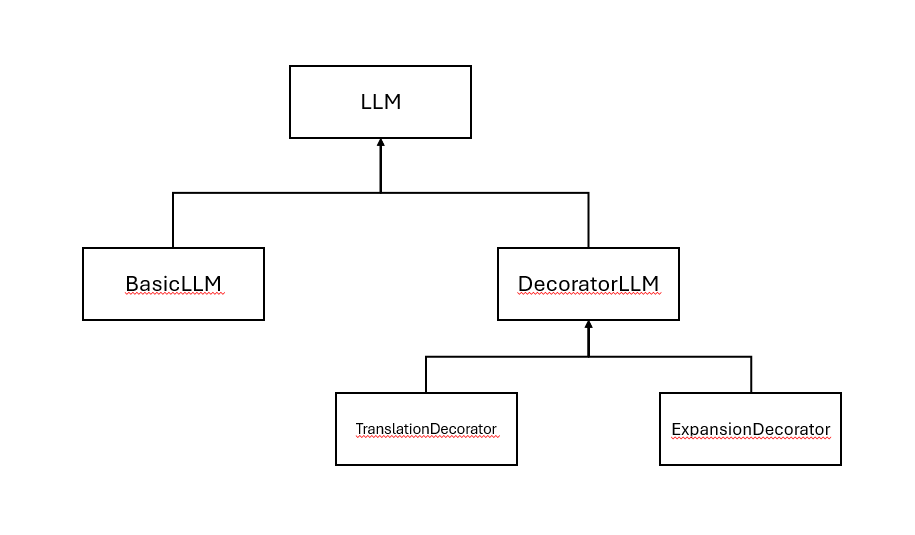
\includegraphics[width=0.75\textwidth]{Images/DiagramaDecorator.png}
    \caption{Diagrama Implementado}
    \label{fig:mi_imagen}
\end{figure}\\

\subsection{Explicación de la implementación}
La implementación de las clases es algo trivial a partir del diagrama anterior, sin embargo hay un par de detalles a recalcar: 
\begin{enumerate}
    \item Se hace uso de la librería \textit{json} para la lectura del archivo de configuración. Esta aporta una forma sencilla de trabajar con los archivos \textit{.json} y de esta forma hacer más sencilla la forma de introducir los parámetros del programa.
    
    \item Se utiliza el cliente de Hugging Face para cada una de las tareas diferentes que realizan los LLMs
    \begin{itemize}
        \item Se utiliza el método \textbf{summarization} para realizar el resumen
        \item El método \textbf{translation} para realizar la traducción
        \item El método \textbf{textgeneration} para la expansión del resumen. En él se limita la entrada a los primeros 250 tokens pues el modelo usado no acepta más
    \end{itemize}
\end{enumerate}

    
\subsection{Resultados obtenidos}
Tras la ejecución del programa con el archivo \textit{config.json} con los parámetros:
\begin{verbatim}
    {
    "texto": "Paris is a city in France full of people and crowded. It is full of tourists because it is one of the most beautiful cities in the world",
    "input_lang": "en",
    "output_lang": "es",
    "model_llm": "facebook/bart-large-cnn",
    "model_translation": "Helsinki-NLP/opus-mt-",
    "model_expansion": "facebook/blenderbot-400M-distill",
    "token": "hf_***************************************"
    }
\end{verbatim}

Se ha obtenido el siguiente resultado: 
\begin{figure}[H] % [h] indica que la imagen debe estar "here" (aquí)
    \centering
    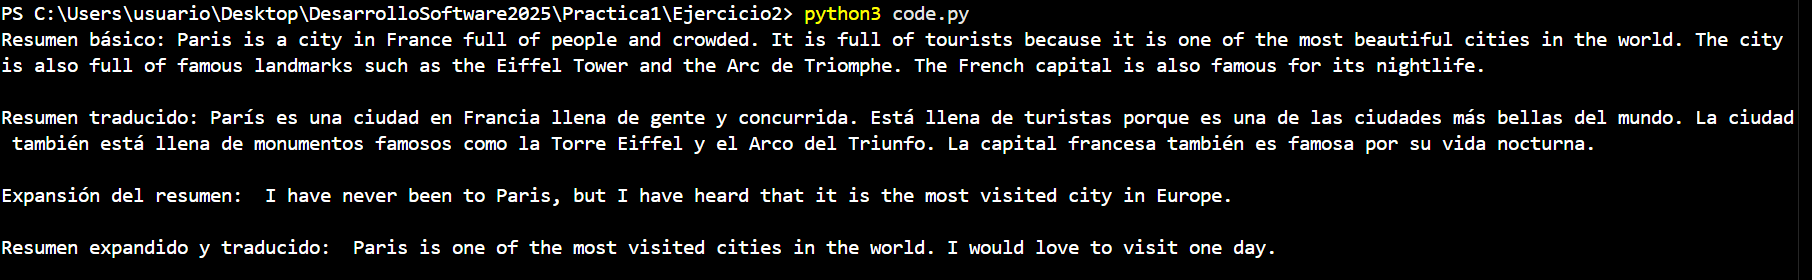
\includegraphics[width=1\textwidth]{Images/salida_programa_e2.png}
    \caption{Salida del Programa}
    \label{fig:mi_imagen}
\end{figure}
\\
En primer lugar se realiza el resumen del texto, para después mostrar su traducción y ampliación. Por último se realiza una composición de la ampliación y traducción. De esta forma, damos por concluido este segundo ejercicio.
\newpage

\section{Ejercicio 3}
\newpage

\section{Ejercicio 4}
\newpage